%------------------------------------------------
\subsection{What is}

\begin{frame}{扩散过程是什么?}

\begin{itemize}
    \item 扩散作用是一个基于分子热运动的输运现象,是分子通过布朗运动从高浓度区域向低浓度区域的运输的过程。它是趋向于热平衡态的驰豫过程,是熵驱动的过程。菲克定律是扩散作用的近似描述,实际过程是从高化学势区域向低化学势区域的转移。
    \item 网络上的扩散过程通常认为是网络上随机游走的极限近似。随机游走的不变分布刻画了网络很多本质的性质。与之对应,扩散过程在大型复杂网络上起到了至关重要的作用。
    \item 由于网络建模的广泛应用,扩散过程以及对应的很多方法也起到了越来越重要的作用,比如相互作用和意见,也可以用来提取关于网络中重要实体或密集实体群的信息。
\end{itemize}

\end{frame}

%------------------------------------------------
\subsection{Fun facts}

\begin{frame}{有趣的例子}
\begin{itemize}
    \item 网络上二维的随机游走是常返的(即从任意一点出发总能以概率为$1$回到原点),而三维的随机游走是非常返的(最终能回到出发点的概率只有大约 34\% )\begin{itemize}
        \item \textit{A drunk man will find his way home, but a drunk bird may get lost forever.} Shizuo Kakutani
    \end{itemize}
    \item 投票模型(Voter Model)中,所有人统一到同一个意见的概率等价于网络的常返概率。
\end{itemize}
\begin{figure}
    \centering
    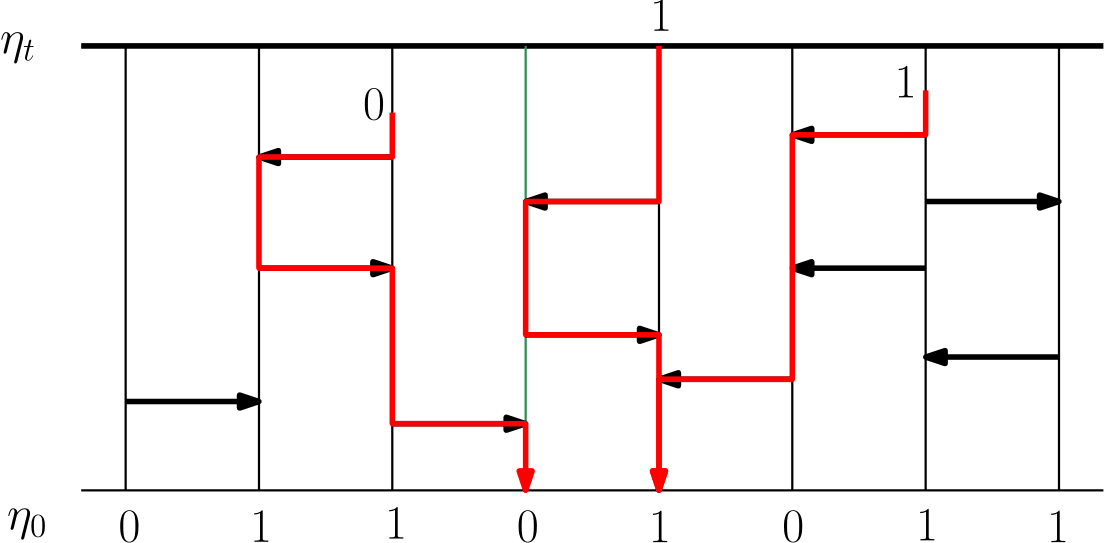
\includegraphics[width = 0.5\linewidth]{PKU_Slide/chaps/voter.png}
    \caption{Voter Consensus versus Random Walk (sourced Wikipedia)}
    % \label{fig:my_label}
\end{figure}
\end{frame}

\begin{frame}{Key factors}

\begin{enumerate}
    \item 网络异质性(尤其是度关联性,群落结构)
    \item 转移概率的定义(决定平稳分布和平均首次通过时间)
    \item 相关的算法(PageRank,特征向量中心性)
    \item 谱性质(我们研究的重点)
\end{enumerate}
    
\end{frame}